\input{configuration}

\title{Lecture 24 --- Concurrency Control }

\author{Jeff Zarnett \\ \small \texttt{jzarnett@uwaterloo.ca}}
\institute{Department of Electrical and Computer Engineering \\
  University of Waterloo}
\date{\today}


\begin{document}

\begin{frame}
  \titlepage

 \end{frame}


\begin{frame}
\frametitle{Concurrency Control}

We now turn our attention to the question of how the database will control the various concurrent elements to make sure that execution goes as planned. 

There are a variety of schemes, but at this point the ones we will examine will always assume that failure does not happen. 

\begin{center}
	
\includegraphics[width=0.4\textwidth]{images/couldgowrong.jpg}
\end{center}

 \end{frame}


\begin{frame}
\frametitle{Concurrency Control}

Once we understand the concurrency control mechanisms we can then build on them to include failure recovery.

\begin{center}
	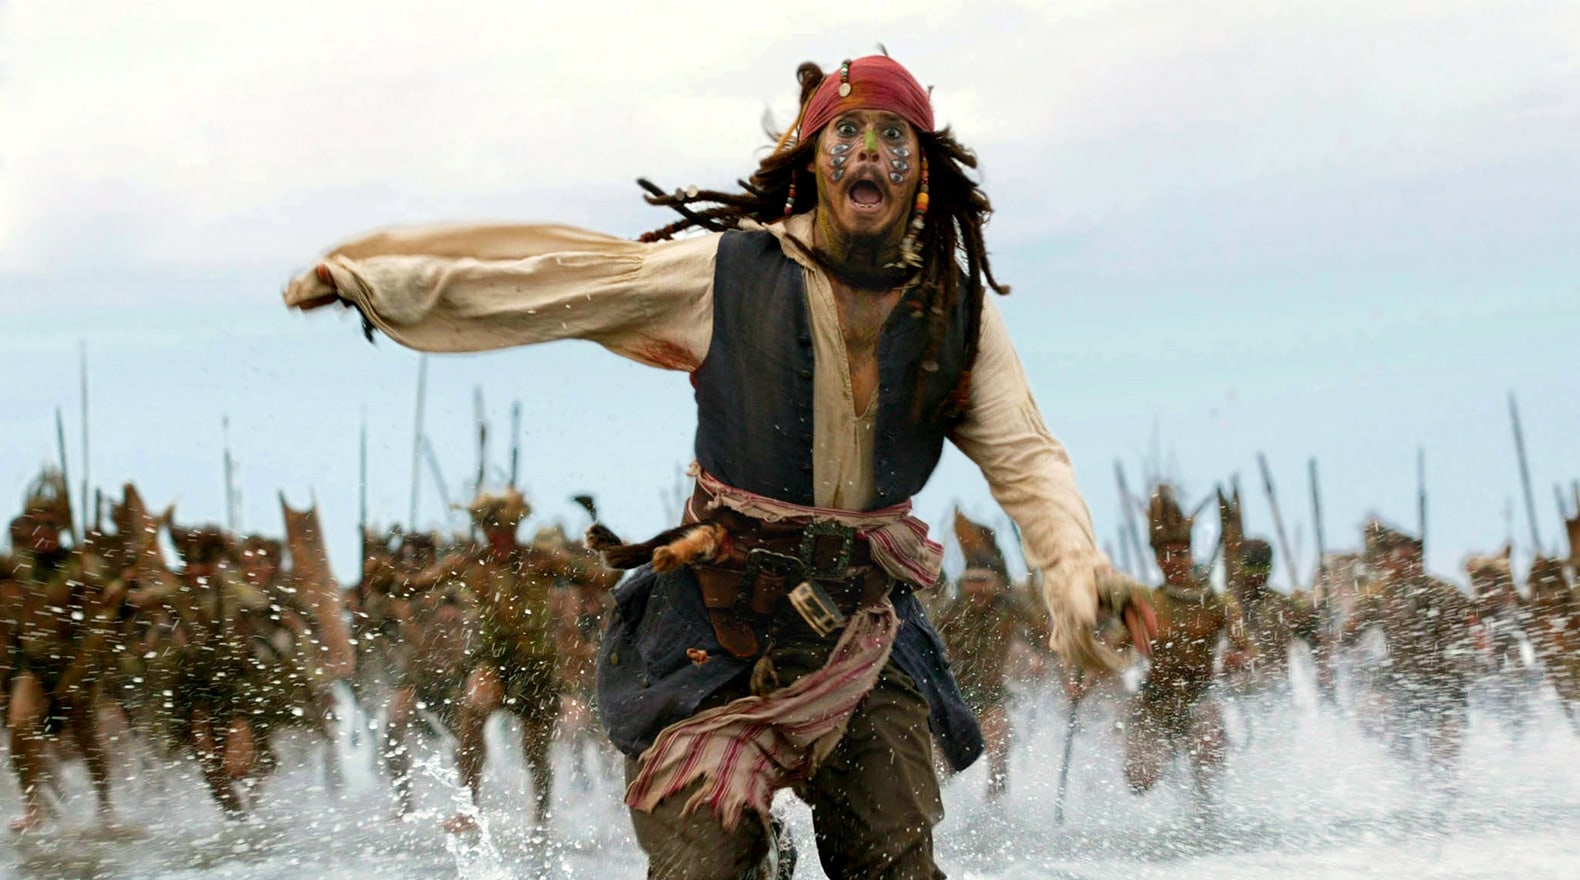
\includegraphics[width=0.5\textwidth]{images/sparrow-run.jpg}
\end{center}

\end{frame}

\begin{frame}
\frametitle{No Concurrency Control}

It is possible from the point of view of the database to simply choose not to implement concurrency control of any sort. 

This is easy for the database designers and effectively means putting the problem of concurrency management in the hands of the users of the database.

\end{frame}

\begin{frame}
\frametitle{Lock-Based Protocols}

Our typical strategy for concurrency problems is locking of some sort. 

You are surely familiar with locks and locking so we will not need to repeat any of the material on that subject from earlier. 

\end{frame}

\begin{frame}
\frametitle{R/W Locks}

For performance reasons we will assume that we use reader/writer type locks. 

There are accordingly two modes in which a data element may be locked: shared mode, and exclusive mode. 

The shared mode lock is denoted by $S$ and exclusive by $X$. 


Every transaction must request a lock before accessing a data item, and the sort of lock it will request depends on what it would like to do.


\end{frame}

\begin{frame}
\frametitle{Requesting Locks}

 The request is made of the concurrency control system and it will either grant the request or delay that transaction until the request is granted.
 
 This you will recognize as being the behaviour of the mutex and semaphore: a requestor may proceed or will be blocked for some period of time.

\end{frame}

\begin{frame}
\frametitle{Your Wish is Granted}

As for whether the request can be granted, this is pretty simple. 

If there are no locks for that item, then the request may be granted. 

If the request is exclusive and there exists any lock on that data item, the request must wait. 


\end{frame}

\begin{frame}
\frametitle{Your Wish is Granted}


If the request is for a read and there exists an exclusive lock on the item, the request must wait. 

If the request is for a read and there exist only read locks on the item, the read may proceed. 

If the request can be granted, that might not guarantee it will be granted immediately.


\end{frame}

\begin{frame}
\frametitle{Wish Granting, Generally}

There could be other lock modes (but we won't consider them in this course).

If so, then we would need to check to see whether a new request's locking mode is compatible with the existing ones. 

The compatibility rule for reader-writer locks is pretty simple as above. 


\end{frame}

\begin{frame}
\frametitle{Wish Granting, Generally}

In the more general approach it is necessary to check all the locks currently held for that item and see if they are compatible. 

If they are all compatible, the lock may be granted.


\end{frame}

\begin{frame}
\frametitle{Remember to Unlock}

As with the kinds of locks we are accustomed to from C-like languages, there is also an unlock operation to, well, unlock that item. 

Unlocking an item will allow some other waiting transaction (or transactions) to be able to then lock that item.

The standard advice in concurrency is to unlock items as soon as possible.

Pay attention to serializability, however...

\end{frame}

\begin{frame}[fragile]
\frametitle{Always Bank Examples}

Suppose there are two concurrent transactions going on. $T_{1}$ is to transfer \$50 from chequing (account C) to savings (account S). 

The second is to show your total net worth.

\end{frame}

\begin{frame}[fragile]
\frametitle{Always Bank Examples}

Let's look at the statements needed to get this done:

\begin{multicols}{2}
\textbf{Transaction $T_{1}$}
\begin{verbatim}
T1.1 Exclusive lock C
T1.2 Read C
T1.3 C = C - 50
T1.4 Write C
T1.5 Unlock C
T1.6 Exclusive Lock S
T1.7 Read S
T1.8 S = S + 50
T1.9 Write S
T1.10 Unlock S
\end{verbatim}

\columnbreak
\textbf{Transaction $T_{2}$}
\begin{verbatim}
T2.1 Shared lock C
T2.2 Read C
T2.3 Unlock C
T2.4 Shared Lock S
T2.5 Read S
T2.6 Unlock S
T2.7 TEMP = A + B
T2.8 Print TEMP


\end{verbatim}
\end{multicols}


\end{frame}

\begin{frame}
\frametitle{More Concurrency, More Problems}

If executed serially we have no problem; we will always get consistent results. 

No matter what order we execute the transactions, the result will be the same since any amount moved from $C$ to $S$ does not affect the total. 

If they are, respectively \$100 and \$200 then the total must remain \$300. 


\end{frame}

\begin{frame}
\frametitle{More Concurrency, More Problems}


If the transactions are executed incorrectly, we will print a result of \$250. 

\begin{center}
	
\includegraphics[width=0.5\textwidth]{images/give-money.png}
\end{center}

How?


\end{frame}

\begin{frame}[fragile]
\frametitle{Solution: Unlock Timing}

The unlocking of elements needs to be delayed appropriately to ensure serializability: 

\begin{multicols}{2}
\textbf{Transaction $T_{1}'$}
\begin{verbatim}
T1.1 Exclusive lock C
T1.2 Read C
T1.3 C = C - 50
T1.4 Write C
T1.5 Exclusive Lock S
T1.6 Read S
T1.7 S = S + 50
T1.8 Write S
T1.9 Unlock C
T1.10 Unlock S
\end{verbatim}

\columnbreak
\textbf{Transaction $T_{2}'$}
\begin{verbatim}
T2.1 Shared lock C
T2.2 Read C
T2.3 Shared Lock S
T2.4 Read S
T2.5 TEMP = A + B
T2.6 Print TEMP
T2.7 Unlock C
T2.8 Unlock S


\end{verbatim}
\end{multicols}


\end{frame}

\begin{frame}
\frametitle{Hello Deadlock, My Old Friend...}

There are no free lunches, though: the risk of longer-held locks is that there can be, as you guessed... \alert{deadlock}! 

Deadlock, as you will recall, is what happens when two or more transactions (formerly processes) are permanently blocked waiting for one another. 

As before, an unfortunate interleaving of lock and unlock statements can mean that the transactions get stuck. 

\end{frame}

\begin{frame}
\frametitle{Hello Deadlock, My Old Friend...}

Deadlock is bad, but not as bad (we think) as inconsistent states being shown (or worse, saved!). 

If a deadlock occurs, we can detect it and then can do something about it; if an inconsistent state is shown then we may never know about it.


\end{frame}

\begin{frame}
\frametitle{Rule 1: Always Make Rules!}

There are often rules in the system for how transactions behave with respect to locks called the \alert{locking protocol}. 

The locking protocol sets up some rules about when items may be (un)locked.

That reduces the number of possible schedules such that the only allowed schedules are conflict-serializable schedules. 

A schedule is considered legal if it follows all the rules of the locking protocol.

\end{frame}

\begin{frame}
\frametitle{Starvation}

Alongside the risk of deadlock, there is also the possibility of starvation. 

\begin{center}
	
\includegraphics[width=0.35\textwidth]{images/stillstanding.png}
\end{center}

The more locks a particular transaction requires, the more likely it is to have to wait and the higher the risk of starvation.

\end{frame}

\begin{frame}
\frametitle{Take a Number}

A new rule: locks should be granted in order of request.

$T_{i}$ will never have to wait for $T_{j}$ that requested that lock later. 

This is, obviously, in addition to the usual rule that the lock can only be granted when the requested lock mode is compatible with the existing locks, if any. 

\end{frame}

\begin{frame}
\frametitle{Two Phase Locking}

Two phase locking: we try to acquire locks and if we are unsuccessful, release any that we have acquired and try again from the beginning. 

The database two phase locking protocol is a little bit different. 

In this there are two distinct phases: growing and shrinking. 

\end{frame}

\begin{frame}
\frametitle{Two Phase Locking}

In the growing phase a transaction may acquire locks; in the shrinking phase a transaction may release locks but may not obtain any new ones. 

The initial state is the growing phase and as soon as the first lock is released then it is not permitted to obtain any new ones

\end{frame}

\begin{frame}
\frametitle{Conflict Serializability}
Any two phase locking protocol gives us, automatically, conflict serializability. 

For any transaction, there exists the point where the last lock has been obtained, and this is called the \alert{lock point}. 

We can order transactions based on their lock points and it gives a serial ordering of the transactions. 

But that's all it gives us: not any sort of freedom from deadlocks or starvation.


\end{frame}

\begin{frame}
\frametitle{More Restrictive}

There exist two more restrictive locking protocols.

The first is the strict two phase locking protocol, which requires that all exclusive locks are held until the transaction is committed.

This guarantees that no intermediate states are ever made visible.

\end{frame}

\begin{frame}
\frametitle{More Restrictive}

The other is the rigorous two phase locking protocol which requires all locks, no matter the type, to be held all the way until the commit.

With rigorous two phase locking, transactions are easily serialized by commit order.

\end{frame}

\begin{frame}
\frametitle{Transitions!}

We can try to squeeze out some more parallelism by allowing locking to have two more operations. 

A transition from shared to exclusive and from exclusive to shared. 

We still need exclusive lock to modify a value, but we can allow some values to be shared during the execution of the transaction. 


\end{frame}

\begin{frame}
\frametitle{Upgrade and Downgrade}

Moving from a shared to exclusive lock is called an upgrade, and that can only be done during the lock acquisition phase.

 Moving from exclusive down to shared is called a downgrade and it can only be done in the shrinking phase.

An upgrade is like trying to acquire a lock, so it can result in blocking of a transaction.

\end{frame}

\begin{frame}
\frametitle{Upgrade \& Downgrade}

\begin{center}
	
\includegraphics[width=0.5\textwidth]{images/upgrade.jpg}
\end{center}


\end{frame}

\begin{frame}
\frametitle{Lock and Unlock Algorithm}

\begin{enumerate}
	\item Scan the transaction from the beginning moving one statement at a time.
	\item If the next instruction is a read of of an item $i$ and there is no lock on $i$ already, insert an instruction to lock $i$ in shared mode before the read.
	\item Otherwise, if the next instruction is a write of an item $i$ and the item $i$ is not already locked exclusively:
		\begin{enumerate}
			\item If the item is locked in shared mode, insert an instruction to upgrade the lock on $i$ to exclusive mode before the write.
			\item Otherwise the item is not locked, insert an instruction to lock $i$ in exclusive mode before the write.
		\end{enumerate}
	\item At the end of the transaction (commit or abort), insert instructions to unlock all locks that were locked (regardless of mode).
\end{enumerate}


\end{frame}

\begin{frame}
\frametitle{Lock Manager Implementation}

The lock manager is the mysterious part of the database that decides when to grant lock requests, and when to deny them. 

In fact, the lock manager receives the requests to lock and unlock commands. 

The lock manager may return a grant of the lock when it is received, or a denial.


\end{frame}

\begin{frame}
\frametitle{Lock Manager Implementation}


But that answer might not come right away: if a grant cannot be completed right now we can delay it until it can be granted. 

Rejection, however, is fatal to the requester: a rejection means the requesting transaction must be rolled back. 

The unlock requests do not strictly speaking require a response.


\end{frame}

\begin{frame}
\frametitle{Lock Tables: Linked List Approach}

Each data element is associated with a linked list. 



\begin{center}
	\includegraphics[width=0.4\textwidth]{images/lock-table}
\end{center}


\end{frame}

\begin{frame}
\frametitle{Lock Table Rules}

Each (lockable) data item is associated with a linked list. 

Entries in that linked list contain the transaction identifier and an flag to indicate granted or waiting.

If a request arrives for a data item for which there is no lock, then an entry is created and the request be immediately granted. 

\end{frame}

\begin{frame}
\frametitle{Lock Table Rules}
If a lock already exists for that data item, a new entry is created. 

As for whether it is granted right away or not, compatibility must be checked. 

If it is compatible it may be granted; otherwise it must wait. 

\end{frame}

\begin{frame}
\frametitle{Lock Table Rules}

When there is an unlock request, the entry for that transaction and data item are removed and, if possible, further requests are granted. 

If a transaction aborts, any locks (granted/not) are removed from the lock table.

\end{frame}

\begin{frame}
\frametitle{Graph Protocol}

The graph based protocol is lock based protocol that uses a tree. 

To make this work, all data elements need to be assigned an identifier which allows establishment of partial ordering on the data elements. 

Why? So it is possible to enforce the rule that they are acquired in order.


\end{frame}

\begin{frame}
\frametitle{Graph (Tree) Protocol}

The tree protocol works only for exclusive locks with four rules:

\begin{enumerate}
	\item The first lock by a transaction $T_{1}$ may be on any data item.
	\item Any other data item $d$ may be locked by $T_{i}$ only if the parent of $d$ is currently locked by $T_{i}$.
	\item Items may be unlocked at any time.
	\item A data item that has been locked and then unlocked by $T_{i}$ cannot later be locked again by $T_{i}$.
\end{enumerate}

\end{frame}


\begin{frame}
\frametitle{Graph (Tree) Protocol}

The diagram below illustrates a potential ordering of data elements:

\begin{center}
\includegraphics[width=0.5\textwidth]{images/tree-lock}
\end{center}

\end{frame}


\begin{frame}
\frametitle{Proof of No Circular Wait}

Assume a circular wait is present. 

Let the set of processes in the circular wait be $\{T_{0}, T_{1}, ... T_{n}\}$ and the set of resources (data elements locked) be $\{R_{0}, R_{1}, ... R_{n}\}$. 

The cycle is formed as: $T_{i}$ is waiting for resource $R_{i}$ and that resource is held by $T_{i+1}$. 

The exception is the case of $T_{n}$, which is waiting for resource $R_{n}$ that is held by $T_{0}$ (completing the cycle by wrapping around). 

\end{frame}


\begin{frame}
\frametitle{Proof of No Circular Wait}


Since Process $T_{i+1}$ holds resource $R_{i}$ while requesting $R_{i+1}$, this means $f(R_{i}) < f(R_{i+1})$ for all $i$. 

But this means that $f(R_{0}) < f(R_{1}) < ... < f(R_{n}) < f(R_{0})$. 

It cannot be the case that $f(R_{0}) < f(R_{0})$: a contradiction, meaning a circular wait cannot occur.


\end{frame}

\begin{frame}
\frametitle{Problems with the Tree}

Use of the tree structured protocol does not, however, ensure recoverability or prevent cascades from occurring. 

That means we need to also take steps, as earlier, to ensure that the schedule conforms to our other properties. 

The other negative here is that the database server might need to lock items other than the ones strictly necessary in the transaction.


\end{frame}

\begin{frame}
\frametitle{Fix It If We Must...}

The tree protocol is useful if the goal is to prevent deadlock from happening, but it is not a very good solution given the tradeoffs.

\begin{center}
	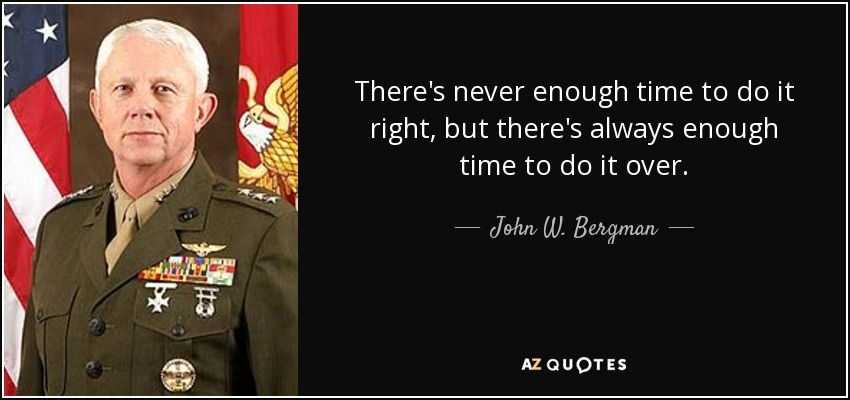
\includegraphics[width=0.75\textwidth]{images/doitover.jpg}
\end{center}

It is more likely that we will just allow transactions to proceed and detect if they do get stuck, and if so, try to do something to fix it.



\end{frame}


\end{document}

